%
% FH Technikum Wien
% !TEX encoding = UTF-8 Unicode
%
% Erstellung von Master- und Bachelorarbeiten an der FH Technikum Wien mit Hilfe von LaTeX und der Klasse TWBOOK
%
% Um ein eigenes Dokument zu erstellen, müssen Sie folgendes ergänzen:
% 1) Mit \documentclass[..] einstellen: Master- oder Bachelorarbeit, Studiengang und Sprache
% 2) Mit \newcommand{\FHTWCitationType}.. Zitierstandard festlegen (wird in der Regel vom Studiengang vorgegeben - bitte erfragen)
% 3) Deckblatt, Kurzfassung, etc. ausfüllen
% 4) und die Arbeit schreiben (die verwendeten Literaturquellen in Literature.bib eintragen)
%
% Getestet mit TeXstudio mit Zeichenkodierung ISO-8859-1 (=ansinew/latin1) und MikTex unter Windows
% Zu beachten ist, dass die Kodierung der Datei mit der Kodierung des paketes inputenc zusammen passt!
% Die Kodierung der Datei twbook.cls MUSS ANSI betragen!
% Bei der Verwendung von UTF8 muss dnicht nur die Kodierung des Dokuments auf UTF8 gestellt sein, sondern auch die des BibTex-Files!
%
% Bugreports und Feedback bitte per E-Mail an latex@technikum-wien.at
%
% Versionen
% *) V0.7: 9.1.2015, RO: Modeline angepasst und verschoben
% *) V0.6: 10.10.2014, RO: Weitere Anpassung an die UK
% *) V0.5: 8.8.2014, WK: Literaturquellen überarbeitet und angepasst
% *) V0.4: 4.8.2014, WK: Initalversion in SVN eingespielt
%
\documentclass[MMR,Master,english]{twbook}
\usepackage[utf8]{inputenc}
\usepackage[T1]{fontenc}
%
% Hier biblatex & Biber konfigurieren; Vergessen Sie nicht, dass Sie biber verwenden müssen um eine Bibliothek zu erzeugen
%
\usepackage[backend=biber, style=numeric, sorting=none]{biblatex}
\addbibresource{Literature.bib}
%
% Bei Bedarf bitte hier die Syntax-Highlightings anpassen
%
% own 
\usepackage{hyperref}
\usepackage{float}
\usepackage{comment}
\usepackage{csquotes}
\usepackage{pgfplots}
\usepackage{soul}
\usepackage{color}
\usepackage{xcolor}  % Required for custom colors
\sethlcolor{blue}
%
% Platzierungsoptionen 
%
\usepackage[final]{listings}
\lstset{captionpos=b, numberbychapter=false,caption=\lstname,frame=single, numbers=left, stepnumber=1, numbersep=2pt, xleftmargin=15pt, framexleftmargin=15pt, numberstyle=\tiny, tabsize=3, columns=fixed, basicstyle={\fontfamily{pcr}\selectfont\footnotesize}, keywordstyle=\bfseries, commentstyle={\color[gray]{0.33}\itshape}, stringstyle=\color[gray]{0.25}, breaklines, breakatwhitespace, breakautoindent}
\lstloadlanguages{[ANSI]C, C++, [gnu]make, gnuplot, Matlab}

%Formatieren des Quellcodeverzeichnisses
\makeatletter
% Setzen der Bezeichnungen für das Quellcodeverzeichnis/Abkürzungsverzeichnis in Abhängigkeit von der eingestellten Sprache
\providecommand\listacroname{}
\@ifclasswith{twbook}{english}
{%
    \renewcommand\lstlistingname{Code}
    \renewcommand\lstlistlistingname{List of Code}
    \renewcommand\listacroname{List of Abbreviations}
}{%
    \renewcommand\lstlistingname{Quellcode}
    \renewcommand\lstlistlistingname{Quellcodeverzeichnis}
    \renewcommand\listacroname{Abkürzungsverzeichnis}
}
% Wenn die Option listof=entryprefix gewählt wurde, Definition des Entyprefixes für das Quellcodeverzeichnis. Definition des Macros listoflolentryname analog zu listoflofentryname und listoflotentryname der KOMA-Klasse
\@ifclasswith{scrbook}{listof=entryprefix}
{%
    \newcommand\listoflolentryname\lstlistingname
}{%
}
\makeatother
\newcommand{\listofcode}{\phantomsection\lstlistoflistings}

% Die nachfolgenden Pakete stellen sonst nicht benötigte Features zur Verfügung
\usepackage{blindtext}
%
% Einträge für Deckblatt, Kurzfassung, etc.
%
\title{Virtualisierung eines Echtzeit-Betriebssystems zur Steuerung eines Roboters mit Schwerpunkt auf die
Einhaltung der Echtzeit}
\author{Halil Pamuk, BSc}
\studentnumber{51842568}
%\author{Titel Vorname Name, Titel\and{}Titel Vorname Name, Titel}
%\studentnumber{XXXXXXXXXXXXXXX\and{}XXXXXXXXXXXXXXX}
\supervisor{Sebastian Rauh, MSc. BEng}
%\supervisor[Begutachter]{Titel Vorname Name, Titel}
%\supervisor[Begutachterin]{Titel Vorname Name, Titel}
%\secondsupervisor{Titel Vorname Name, Titel}
%\secondsupervisor[Begutachter]{Titel Vorname Name, Titel}
%\secondsupervisor[Begutachterinnen]{Titel Vorname Name, Titel}
\place{Wien}
\kurzfassung{Erstellung einer Echtzeit-Robotersteuerungsplattform unter Verwendung von Salamander OS, Xenomai, QEMU
und PCV-521 in der Yocto-Umgebung. Die Plattform basiert auf Salamander OS und nutzt Xenomai für Echtzeit-
Funktionen. Dazu muss im ersten Schritt die Virtualisierungsplattform evaluiert werden. (QEMU, Hyper-V, Virtual
Box, etc.) Als weiterer Schritt folgt die Anbindung eines Roboters über eine VARAN-Bus Schnittstelle. Das
gesamte System wird in der Yocto-Umgebung erstellt und konfiguriert.
Das Hauptziel der Arbeit ist es, herauszufinden, wie die Integration von Echtzeit-Funktionen und effizienten
Kommunikationssystemen in eine Robotersteuerungsplattform die Reaktionszeit und Zuverlässigkeit von
Roboteranwendungen verbessern kann}
\schlagworte{Schlagwort1, Schlagwort2, Schlagwort3, Schlagwort4}
\outline{Abstract}
\keywords{Echtzeit, Virtualisierung, Xenomai, VARAN}
%\acknowledgements{\blindtext}

\begin{document}

\maketitle

%
% .. und hier beginnt die eigentliche Arbeit. Viel Erfolg beim Verfassen!
%
%Die folgende Gliederung von Bachelor- und Masterarbeiten ist für die Robotik-Studiengänge
%verpflichtend vorgeschrieben.
%
%- Deckblatt
%- Eidesstattliche Erklärung (digital signiert)
%- Kurzfassung und Abstract mit Schlüsselwörtern/Keywords
%- Danksagung (optional)
%- Inhaltsverzeichnis

%- Einleitung (die genannten Punkte müssen keine eigenen Unterkapitel sein, müssen aber aus der Einleitung klar hervorkommen):
%   - Stand der Technik
%   - Problem- und Aufgabenstellung
%   - Zielsetzung
%- Hauptteil -> Gliederung je nach Thema
%   - Methodik
%   - Resultate
%   - Wirtschaftliche Betrachtung (optional)
%   - Diskussion
%- Zusammenfassung und Ausblick

%- Literaturverzeichnis
%- Abbildungsverzeichnis
%- Tabellenverzeichnis
%- Abkürzungsverzeichnis (optional)
%- Glossar (optional)
%- Anhang (optional)
\chapter{Introduction}\label{cha:introduction}
In today's industrial production and automation, robot systems are well established and of crucial importance. Robots must react to their environment and perform time-critical tasks within strict time constraints. Delays or errors can have catastrophic consequences in some cases. Traditional operating systems, such as Windows or Linux, are often not suitable for these types of real-time requirements as they cannot guarantee deterministic execution times. Therefore, real-time operating systems are required that are specifically designed to react to events within fixed time limits and prioritise the execution of high-priority processes.

\bigskip \noindent The core component of an RTOS that enables real-time capabilities is the kernel. The kernel is responsible for managing system resources, scheduling tasks, and ensuring deterministic behavior. It employs preemptive scheduling mechanisms to allow high-priority tasks to preempt lower-priority tasks, ensuring that time-critical tasks are not delayed. The kernel also implements priority-based scheduling algorithms, such as Rate Monotonic Scheduling (RMS) or Earliest Deadline First (EDF), to schedule tasks based on their priorities and timing constraints. Additionally, RTOS kernels are designed to minimize interrupt latency, which is crucial for real-time applications that require immediate response to external events.

\bigskip \noindent In these RTOS systems, task scheduling is based on so-called priority-based preemptive scheduling. Each task in a software application is assigned a priority. A higher priority means that a faster response is required. Preemptive task scheduling ensures a very fast response. Preemptive means that the scheduler can stop a currently running task at any point if it recognizes that another task needs to be executed immediately. The basic rule on which priority-based preemptive scheduling is based is that the task with the highest priority that is ready to run is always the task that must be executed. So if both a task with a lower priority and a task with a higher priority are ready to run, the scheduler ensures that the task with the higher priority runs first. The lower priority task is only executed once the higher priority task has been processed. Real-time systems are usually categorized as either soft or hard real-time systems. The difference lies exclusively in the consequences of a violation of the time limits.

\bigskip \noindent Hard real-time is when the system stops operating if a deadline is missed, which can have catastrophic consequences. Soft real-time exists when a system continues to function even if it cannot perform the tasks within a specified time. If the system has missed the deadline, this has no critical consequences. The system continues to run, although it does so with undesirably lower output quality.

\clearpage
\section{Application Context}
This master's thesis was written at SIGMATEK GmbH \& Co KG \cite{pixelartSIGMATEKKompletteAutomatisierungssysteme}.
%This section provides necessary information about the starting point and boundary conditions of the thesis, as the work should be reproducible with the means used. 
SIGMATEK uses its own customized Linux distribution to be run on their self-manufactured CPUs, namely Salamander 4. This operating system employs hard real-time with latency requirements between 20 and 50 \textmu s. The goal is to virtualize Salamander 4 and approach the performance of bare metal CPUs. Salamander 4 is virtualized through a third party service, QEMU. The details of this operating system are explained in chapter \ref{cha:salamander4}.



\clearpage
\section{State of the art}
\clearpage
\section{Problem and task definition}
\clearpage
\section{Objective}

The main objective of this work is to create a real-time robot control platform that integrates Salamander OS, Xenomai, QEMU and PCV-521 in the Yocto environment.


%%%%%%%%%%%%%%%%%%%%%%%%%%%%%%%%%%%%%%%%%%%%%%%%%%%%%%%%%%
\clearpage

\chapter{Methodology}\label{cha:methodology}

This section describes in detail all the theoretical concepts and boundary conditions as well as practical methods that contributed to achieving the objectives of this master's thesis.


\begin{comment}

Zu Beginn der Arbeit wurde eine ausführliche Analyse der einzelnen Virtualisierungsmöglichkeiten von Salamander 4 durchgeführt. Im Besonderen wurde hier die Virtualisierungsperformance von Ubuntu 22.04, Windows 10 und WSL unter QEMU verglichen.

First, a comprehensive literature review is conducted to understand the current trends and challenges in real-time robot control. Based on the literature study, a suitable virtualisation platform is selected.


After the selection of the virtualisation platform, the robot control platform is implemented. This step includes the installation and configuration of Salamander OS, Xenomai, QEMU and PCV-521 in the Yocto environment. Once the platform has been implemented, the robot is connected via a VARAN bus interface. Finally, the platform is evaluated to determine how the integration of real-time functions and efficient communication systems improves the response time and reliability of robot applications.

- Evaluation der Virtualisierungsplattform:
Ich werde verschiedene Virtualisierungsplattformen wie QEMU, Hyper-V, Virtual Box usw. evaluieren. Dies ist ein wichtiger Schritt, um die beste Plattform für meine Anforderungen zu finden.

- Erstellung und Konfiguration des Systems in der Yocto-Umgebung:
Ich werde das Yocto-Framework verwenden, um mein Embedded Linux System zu erstellen und zu konfigurieren. Yocto bietet viele Tools und Funktionen, die mir bei der Erstellung und Konfiguration meines Systems helfen können.


- Anbindung eines Roboters über eine VARAN-Bus Schnittstelle:
Ich plane, einen Roboter in mein System zu integrieren. Ich werde eine VARAN-Bus Schnittstelle verwenden, um eine schnelle und zuverlässige Kommunikation zwischen dem Roboter und dem Steuerungssystem zu gewährleisten.

\end{comment}

\bigskip \noindent Trace-cmd was used for tracing the Linux kernel. It can record various kernel events such as interrupts, scheduler decisions, file system activity, function calls in real time. Trace-cmd helped in getting detailed insights into system behaviour and identify reasons for latency \cite{Tracecmd}.

\bigskip \noindent The data that was recorded by trace-cmd was then fed into Kernelshark, which is a graphical front-end tool \cite{KernelShark}. It visualizes the recorded kernel trace data in a readable way on an interactive timeline, which facilitated the process of identifying patterns and correlations between events. By further filtering the displayed events according to specific criteria such as processes, event types or time ranges, the latency issues were analyzed.

\bigskip \noindent Real-time operating system capabilities were provided by Xenomai, which is real-time development framework that extends the Linux kernel. It enables low-latency and deterministic execution of time-critical tasks. Xenomai introduces a dual-kernel approach with a real-time kernel coexisting alongside Linux. A key utility within the Xenomai suite is the latency tool, which benchmarks the timer latency - the time it takes for the kernel to respond to timer interrupts or task activations. The tool creates real-time tasks or interrupt handlers and measures the latency between expected and actual execution times \cite{XenomaiXenomai}.

\clearpage

\chapter{Salamander 4}\label{cha:salamander4}
This chapter breifly describes the Salamander 4 operating system by SIGMATEK.

Salamander 4 is the proprietary operating system of SIGMATEK. It is based on Linux version 5.15.94 and integrates Xenomai 3.2, a real-time development environment \cite{XenomaiXenomai}. Salamander 4 is a 64-bit system, which refers to the x86\_64 architecture. The real-time behaviour is achieved through the use of Symmetric Multi-Processing (SMP) and Preemptive Scheduling (PREEMPT). In addition, it uses IRQPIPE to process interrupts in a way that meets the real-time requirements of the system. The output of the command \texttt{uname -a} can be observed in code \ref{output:uname_a}.

\vspace{1em}
\begin{minipage}{0.95\columnwidth}
	\begin{lstlisting}[name={System information},label={output:uname_a}]
root@sigmatek-core2:~# uname -a
Linux sigmatek-core2 5.15.94 #1 SMP PREEMPT IRQPIPE Tue Feb 14 18:18:05 UTC 2023 x86_64 GNU/Linux
\end{lstlisting}
\end{minipage}

\noindent Salamander 4 is powered by SIGMATEK's CPU and is comprised of the following software modules:

 \begin{itemize}
	\item \textbf{Operating system}
	\item \textbf{Loader}
	\item \textbf{Hardware classes}
	\item \textbf{Application}
\end{itemize}

\noindent The interfaces between the individual modules are indicated by an arrow in Figure \ref{fig:lasal_cpu}.

\begin{figure}[H]
	\centering
	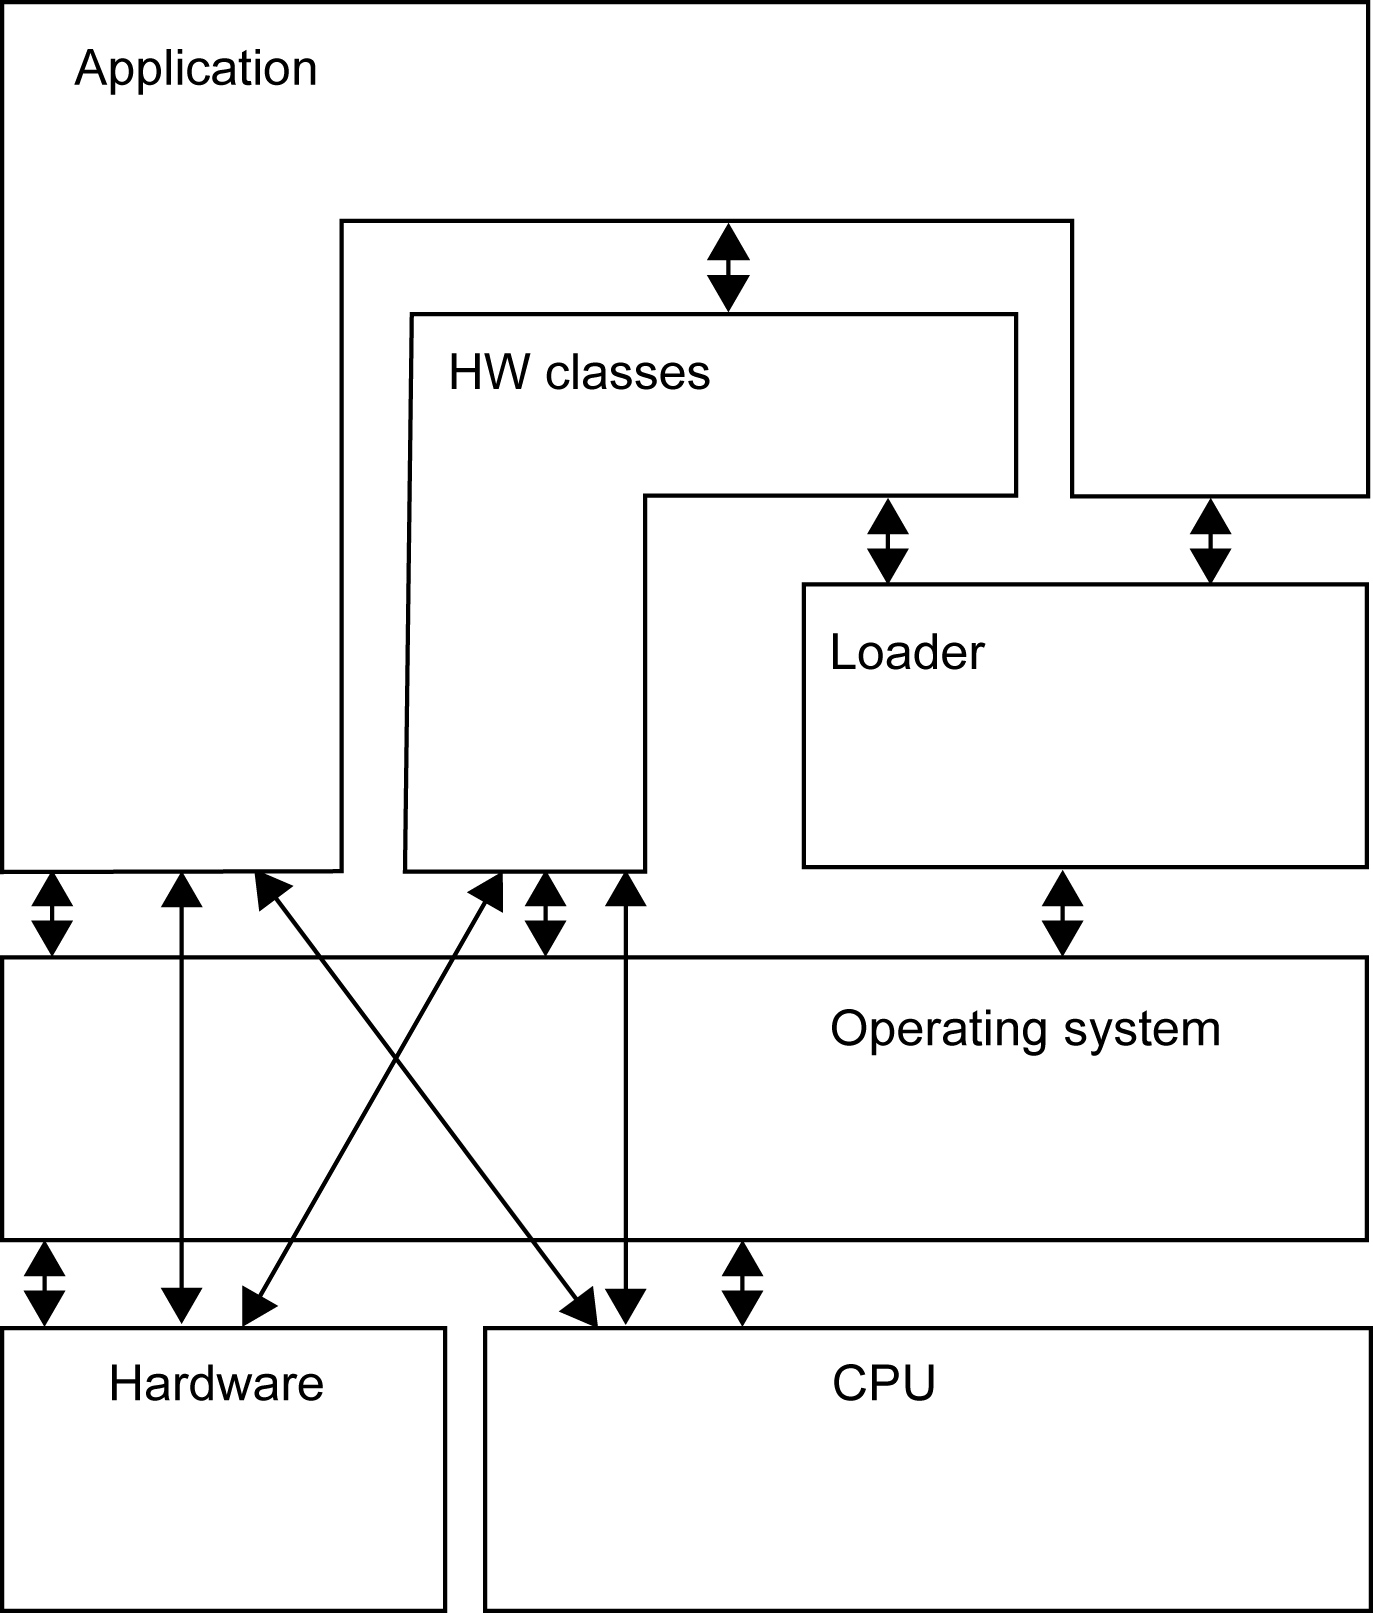
\includegraphics[width=0.8\columnwidth]{img/Software-Struktur_einer_LASAL_CPU.png}
	\caption[LASAL CPU]{LASAL CPU}
	\label{fig:lasal_cpu}
\end{figure}
\clearpage
\section{Xenomai}

\noindent Xenomai consists of 3 parts. These can be found in the Table \ref{tab:what_is_xenomai}.

\begin{table}[!h]
	\centering
	\caption[Xenomai architecture]{Xenomai architecture}
	\label{tab:what_is_xenomai}
	\setlength{\tabcolsep}{0.5em} % for the horizontal padding
	{\renewcommand{\arraystretch}{1.2}% for the vertical padding
		\begin{tabular}{|c|p{0.6\textwidth}|}
			\hline
			\textbf{Teil}  & \textbf{Beschreibung}                                                                  \\ \hline
			i-pipe         & Kernelerweiterung für das Domain-Konzept                                               \\ \hline
			Xenomai Kernel & Benutzt die i-pipe, und hängt sich als root-Domain ein                                 \\ \hline
			Xenomai User   & Programme (LRT) verwenden diese Bibliothek, um Xenomai Funktionen verwenden zu können. \\ \hline
		\end{tabular}}
\end{table}


\noindent Xenomai beruht auf einem Domain-Konzept, das bedeutet, dass alle IRQ an die erste Domain gesendet werden. (root – Domain / Xenomai)
Nur wenn diese nichts mehr zu tun hat, dann darf die 2. Domain arbeiten.
Das bedeutet, erst wenn alle Xenomai Task in einem Wartezustand sind, arbeiten die Linux-Tasks.

\noindent In der Regel unterbricht der Prozessor beim IRQ-Handling seine aktuellen Aktivitäten, um einen Interrupt zu bearbeiten, während die IRQ-Behandlung von Xenomai einen Interrupt-Pipeline-Mechanismus verwendet, der das gleichzeitige Abrufen und Vorbereiten eines anderen Interrupts ermöglicht, während ein Interrupt bearbeitet wird, was die Leistung verbessert und die Latenzzeit verringert.

\noindent Was Xenomai4 von seinem Vorgänger Xenomai3 unterscheidet, ist die vollständige Neugestaltung der Ausführungsphase mit hoher Priorität. Dies geschah aus Gründen der Portabilität und Wartungsfreundlichkeit: I-pipe - die zweite Iteration der ursprünglichen Adeos-Interrupt-Pipeline - wurde vollständig durch Dovetail ersetzt.

\begin{table}[H]
	\centering
	\caption[Domain specific functions]{Domain specific functions}
	\label{tab:domain_specific_functions}
	\begin{tabular}{|c|c|}
		\hline
		\textbf{Xenomai spezifische Funktionen} & \textbf{Linux spezifische Funktionen} \\ \hline
		Tasks                                   & Dateizugriffe                         \\ \hline
		Mutexes, Semaphoren, Events             & Netzwerk                              \\ \hline
	\end{tabular}
\end{table}


\noindent Ein Aufruf dieser Funktionen erfordert die entsprechende Domain. Wenn der Task in der falschen Domain läuft, dann wird ein Domain-Wechsel forciert.
Ein Domainwechsel von Xenomai nach Linux geht relativ einfach. Aber der Wechsel von Linux nach Xenomai braucht Unterstützung, und dafür ist die Hilfe des Gatekeepers notwendig. Das bedeutet, der Gatekeeper hilft einem Task von Linux nach Xenomai zu wechseln.

\clearpage
\section{Task priorities}
Es gibt grundsätzlich 4 Gruppen

\begin{table}[ht]
	\centering
	\caption{Overview of the priority groups and their relationships}
	\label{tab:priorities}
	\begin{tabular}{|c|c|}
		\hline
		\textbf{Prioritätsgruppe}    & \textbf{Bereich} \\ \hline
		Xenomai Priorität            & 0 bis 99         \\ \hline
		Linux RT Priorität           & 1 bis 99         \\ \hline
		Linux (Nice Level) Priorität & -20 bis 19       \\ \hline
		RTK Priorität                & 0 bis 14         \\ \hline
	\end{tabular}
\end{table}
\clearpage
\section{Memory Management}
Es gibt verschiedene Speicherbereiche

Linux/System/Programm Speicher
Der Speicher, den Linux und Programme belegt haben.
Dieser Speicher ist intern in viele Teile aufgeteilt. (DMA, …)

LRT-Heap Speicher
Speicher den der LRT verwendet, oder welcher über ein CIL Funktionen
angefordert wird.

App Heap, App Code, …


\begin{figure}[H]
	\centering
	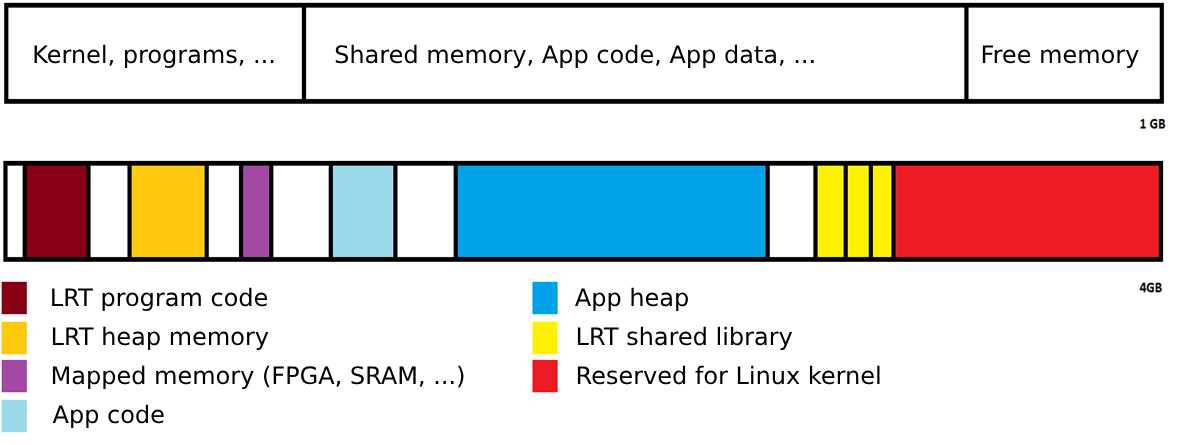
\includegraphics[width=0.8\columnwidth]{img/RAM_Memory_management.png}
	\caption[Memory Management]{Memory Management}
	\label{fig:memory_management}
\end{figure}

\clearpage

\chapter{Initial Real-Time Latency}\label{cha:initial-real-time-latency}

\clearpage
\section{Salamander 4 Bare Metal}
Salamander 4 Bare Metal refers to the proprietary hardware of SIGMATEK used to employ the custom operating system, including

Figure \ref{fig:max_latency_hardware} shows latency of hardware Salamander4.
\begin{figure}[H]
	\centering
	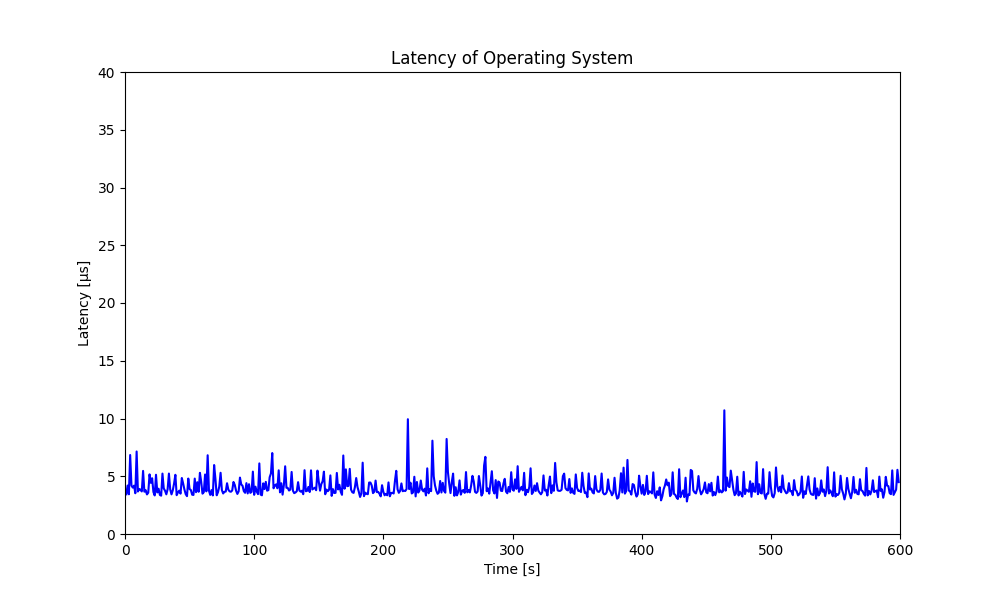
\includegraphics[width=0.8\columnwidth]{img/max_latency_hardware.png}
	\caption[Latency hardware]{Latency hardware}
	\label{fig:max_latency_hardware}
\end{figure}
\clearpage
\section{Salamander 4 Virtualisation}
In addition to providing Salamander 4 on its own hardware, SIGMATEK has also developed a virtualised version of this operating system. It was developped using Yocto, an open source project that allows customised Linux distributions to be created for embedded systems \cite{WelcomeYoctoProject}. The virtualisation runs in a QEMU environment, which is an open source tool for hardware virtualisation \cite{QEMU}. With the help of the script depicted in code \ref{script:qemu_def}, Salamander 4 is started together with the necessary hardware components in the QEMU environment. This makes it possible to run Salamander 4 on a variety of host systems, regardless of the specific hardware of the host. Upon generating the necessary files, Yocto generates a QEMU folder with the following components shown in code \ref{lst:ls}.

\vspace{1em}
\begin{minipage}{\linewidth}
	\begin{lstlisting}[name={Contents of QEMU folder for Salamander 4},label={lst:ls}]
    sigma_ibo@localhost:~/Desktop/salamander-image$ ls -1
    bzImage
    drive-c
    ovmf.code.qcow2
    qemu_def.sh
    salamander-image-sigmatek-core2.ext4
    stek-drive-c-image-sigmatek-core2.tar.gz
    vmlinux
    \end{lstlisting}
\end{minipage}



\vspace{1em}
\begin{minipage}{\linewidth}
	\begin{lstlisting}[name={QEMU script for starting Salamander 4 virtualisation},label={script:qemu_def}]
    #!/bin/sh

    if  [ ! -d drive-c/ ]; then
            echo "Filling drive-c/"
            mkdir drive-c/
            tar -C drive-c/ -xf stek-drive-c-image-sigmatek-core2.tar.gz
    fi
    
    exec  qemu-system-x86_64 -M pc,accel=kvm -kernel ./bzImage \
    -m 2048 -drive file=salamander-image-sigmatek-core2.ext4,format=raw,media=disk \
    -append "console=ttyS0 console=tty1 root=/dev/sda rw panic=1 sigmatek_lrt.QEMU=1 ip=dhcp rootfstype=ext4 schedstats=enable" \
    -net nic,model=e1000,netdev=e1000 -netdev bridge,id=e1000,br=nm-bridge \
    -fsdev local,security_model=none,id=fsdev0,path=drive-c -device virtio-9p-pci,id=fs0,fsdev=fsdev0,mount_tag=/mnt/drive-C \
    -device vhost-vsock-pci,guest-cid=3,id=vsock0 \
    -drive if=pflash,format=qcow2,file=ovmf.code.qcow2 \
    -no-reboot -nographic
\end{lstlisting}
\end{minipage}
\clearpage
Here is a description of the used components:
\begin{itemize}
	\item \textbf{bzImage}: Compressed Linux kernel image, loaded by QEMU at system start.
	\item \textbf{ovmf.code.qcow2}: Firmware file for QEMU, enables UEFI boot process.
	\item \textbf{qemu\_def.sh}: Shell script, starts QEMU with correct parameters to boot Salamamder 4 OS.
	\item \textbf{stek-drive-c-image-sigmatek-core2.tar.gz}: Archive containing files for C drive, unpacked and copied to drive-c/ directory by qemu\_def.sh script.
	\item \textbf{drive-c}: Directory serving as C drive for QEMU system, created and filled by qemu\_def.sh script.
	\item \textbf{salamander-image-sigmatek-core2.ext4}: Root file system for Salamander 4 OS, used as hard drive for QEMU system.
	\item \textbf{vmlinux}: Uncompressed Linux kernel image, typically used for debugging, contains debugging symbols not present in bzImage.
\end{itemize}

%   \begin{table}[ht]
%       \centering
%       \caption{QEMU script components}
%       \label{tab:qemu_components}
%       \begin{tabular}{|l|p{8cm}|}
%           \hline
%           \textbf{File} & \textbf{Description} \\
%           \hline
%           bzImage & Compressed Linux kernel image, loaded by QEMU at system start. \\
%           \hline
%           ovmf.code.qcow2 & Firmware file for QEMU, enables UEFI boot process. \\
%           \hline
%           qemu\_def.sh & Shell script, starts QEMU with correct parameters to boot Salamamder 4 OS. \\
%           \hline
%           stek-drive-c-image-sigmatek-core2.tar.gz & Archive containing files for C drive, unpacked and copied to drive-c/ directory by qemu\_def.sh script. \\
%           \hline
%           drive-c & Directory, serves as C drive for QEMU system, created and filled by qemu\_def.sh script. \\
%           \hline
%           salamander-image-sigmatek-core2.ext4 & Root file system for Salamander 4 OS, used as hard drive for QEMU system. \\
%           \hline
%           vmlinux & Uncompressed Linux kernel image, typically used for debugging, contains debugging symbols not present in bzImage. \\
%           \hline
%       \end{tabular}
%   
%   \end{table}

\noindent When the script is started from the host, the QEMU process can be scheduled to run on any available core, as it is noted bound to a specific CPU core. This means that the QEMU process may frequently switch between different cores, leading to an increase in latency. As the goal was to reduce latency in the guest, the first step was to isolate a CPU of the host and dedicate it solely to the QEMU process, so that it cannot be used for other tasks on user level. However, the isolcpus function only isolates at the user level and does not affect kernel tasks. Consequently, these kernel tasks and interrupts can still utilize the CPU.


Figure \ref{fig:max_latency_default} shows latency of QEMU default Salamander4.

\begin{figure}[H]
	\centering
	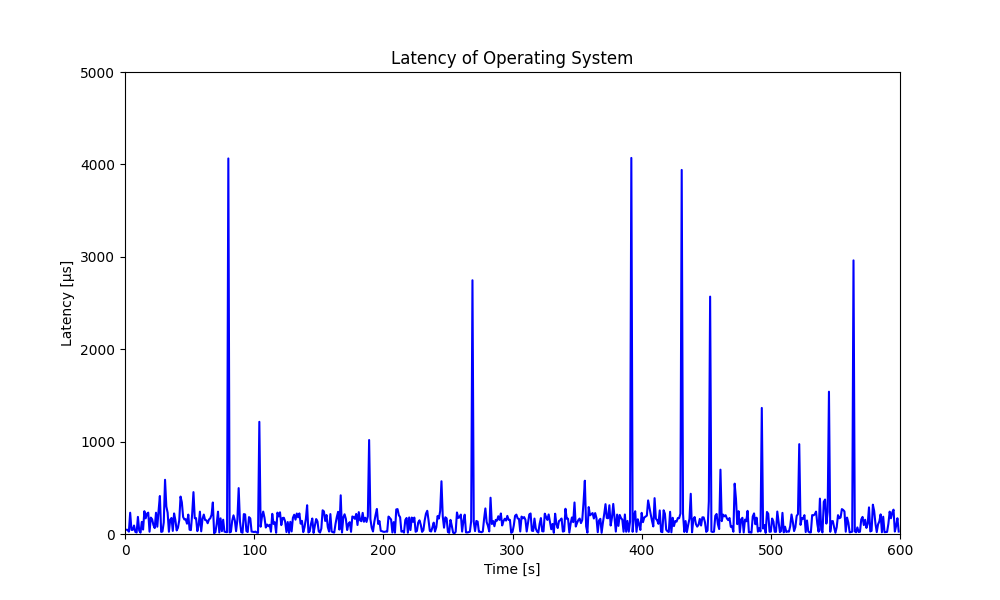
\includegraphics[width=0.75\columnwidth]{img/max_latency_default.png}
	\caption[Latency no taskset]{Latency no taskset}
	\label{fig:max_latency_default}
\end{figure}


Figure \ref{fig:max_latency_taskset} shows latency of QEMU taskset Salamander4.
\begin{figure}[H]
	\centering
	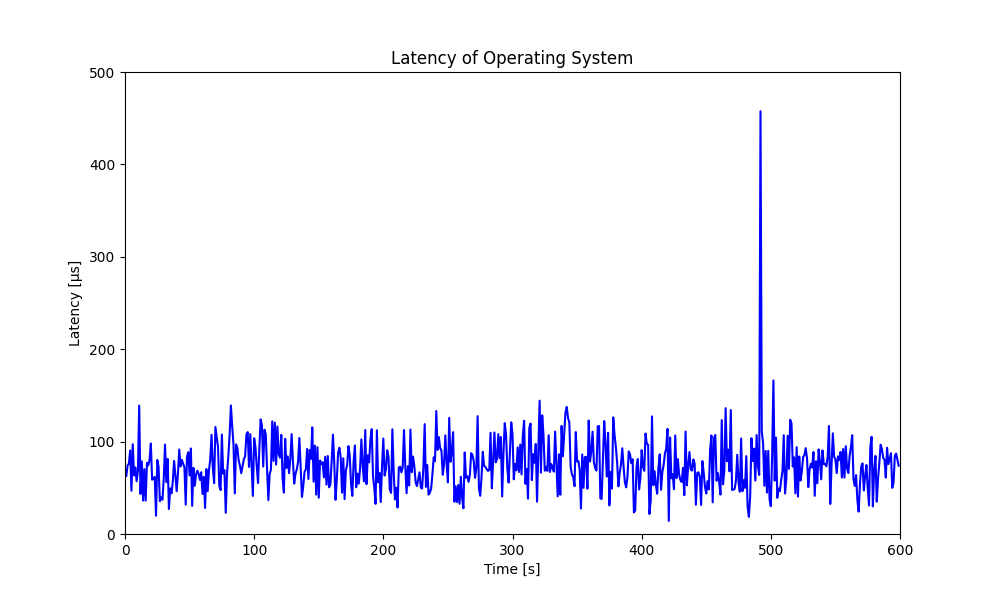
\includegraphics[width=0.75\columnwidth]{img/max_latency_taskset.png}
	\caption[Latency taskset]{Latency taskset}
	\label{fig:max_latency_taskset}
\end{figure}

Figure \ref{fig:max_latency_vapic} shows latency of QEMU vapic Salamander4.
\begin{figure}[H]
	\centering
	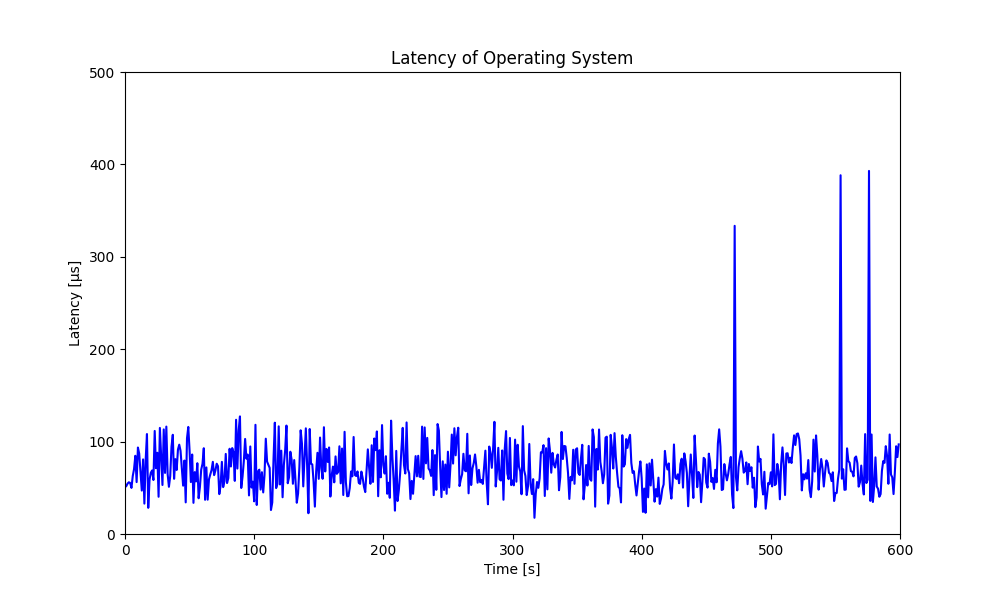
\includegraphics[width=0.75\columnwidth]{img/max_latency_vapic.png}
	\caption[Latency vapic]{Latency vapic}
	\label{fig:max_latency_vapic}
\end{figure}


\noindent Upon isolating a CPU to the QEMU process, it was anticipated that the guest would utilize nearly 100\% of the CPU's capacity, with minimal to no intervention from the host. However, the isolcpus function only isolates at the user level and does not affect kernel tasks. Consequently, these kernel tasks and interrupts can still utilize the CPU. This led to the investigation of the causes for the observed high and inconsistent latency. The guest operates within the kvm\_entry and \texttt{kvm\_exit} events of the host. Kernelshark revealed a high frequency of \texttt{kvm\_exit} events, indicating that the guest frequently relinquishes control of the CPU back to the host. This frequent switching hinders the guest\'s ability to run continuously, thereby increasing the virtualization latency. To further understand this, trace-cmd was employed to trace various events in the host-guest communication, including the reasons for these events. Specifically, the causes for \texttt{kvm\_exit} events were analyzed. The command sudo trace-cmd record -e all -A @3:823 --name Salamander4 -e all was executed on the host for a duration of 5 seconds. The results in Figure \ref{fig:kvm_exit_taskset} were obtained. Additionally, table \ref{tab:kvm_exit} provides a short description of the observed \texttt{kvm\_exit} events.


\begin{table}[H]
	\centering
	\begin{tabular}{|l|p{0.62\textwidth}|}
		\hline
		\textbf{Exit Reason} & \textbf{Description}                                     \\
		\hline
		APIC\_WRITE          & Triggered when the guest writes to its APIC.             \\ \hline
		EXTERNAL\_INTERRUPT  & Triggered by external hardware interrupts.               \\ \hline
		HLT                  & Triggered when the guest executes the HLT instruction.   \\ \hline
		EPT\_MISCONFIG       & Triggered by a misconfiguration in the EPT.              \\ \hline
		PREEMPTION\_TIMER    & Triggered when the host's preemption timer expires.      \\ \hline
		PAUSE\_INSTRUCTION   & Triggered when the PAUSE instruction is executed.        \\ \hline
		EPT\_VIOLATION       & Triggered by a violation of the EPT permission settings. \\ \hline
		IO\_INSTRUCTION      & Triggered when the guest executes an I/O instruction.    \\ \hline
		EOI\_INDUCED         & Triggered when an EOI signal is sent to the APIC.        \\ \hline
		MSR\_READ            & Triggered when the guest reads from a MSR.               \\ \hline
		CPUID                & Triggered when the guest executes the CPUID instruction. \\ \hline
	\end{tabular}
	\caption{Description of kvm\_exit reasons}
	\label{tab:kvm_exit}
\end{table}

\clearpage
Figure \ref{fig:kvm_exit_taskset} shows \texttt{kvm\_exit} frequency with CPU islation.
\begin{figure}[H]
	\centering
	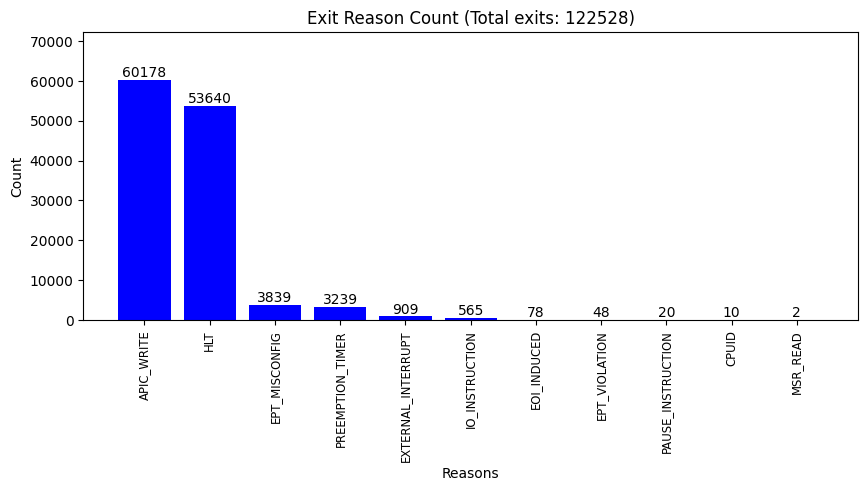
\includegraphics[width=1.0\columnwidth]{img/kvm_exits_taskset.png}
	\caption[kvm exits]{kvm exits}
	\label{fig:kvm_exit_taskset}
\end{figure}

Figure \ref{fig:kvm_exits_default} shows \texttt{kvm\_exit} frequency without CPU islation.
\begin{figure}[H]
	\centering
	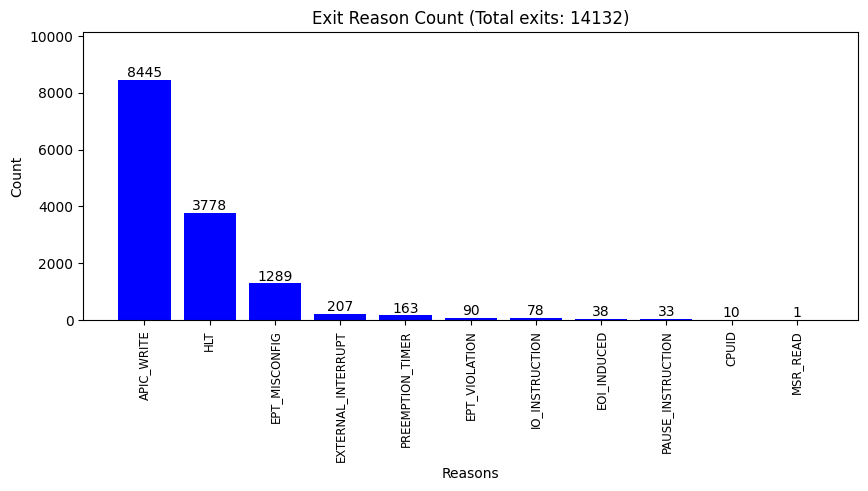
\includegraphics[width=1.0\columnwidth]{img/kvm_exits_default.png}
	\caption[kvm exits default]{kvm exits default}
	\label{fig:kvm_exits_default}
\end{figure}

\clearpage


\begin{table}[h!]
	\centering
	\begin{minipage}{.5\textwidth}
	\centering
	\caption{Host report CPU19 (Total of 445.908)}
	\label{tab:results_host_report}
	\begin{tabular}{|c|c|c|}
	\hline
	PID & Task & Count \\ \hline
	182579 & qemu-system-x86 & 302.748 \\ \hline
	0 & \textless{}idle\textgreater{} & 112.911 \\ \hline
	182618 & vhost & 21.204 \\ \hline
	182572 & qemu-system-x86 & 7.597 \\ \hline
	182755 & qemu-system-x86 & 644 \\ \hline
	182754 & qemu-system-x86 & 643 \\ \hline
	181870 & kworker/19:1 & 139 \\ \hline
	3820 & kworker/19:1H & 16 \\ \hline
	94 & migration/19 & 6 \\ \hline
	\end{tabular}
	\end{minipage}%
	\begin{minipage}{.5\textwidth}
	\centering
	\caption{Guest report (Total of 362.370)}
	\label{tab:results_guest_report}
	\begin{tabular}{|c|c|c|}
	\hline
	PID & Task & Count \\ \hline
	0 & \textless{}idle\textgreater{} & 150.744 \\ \hline
	331 & LRT-Main & 56.697 \\ \hline
	377 & trace-cmd & 48.507 \\ \hline
	346 & CLI & 26.426 \\ \hline
	378 & kthreadd & 25.837 \\ \hline
	340 & MainTaskLow & 19.291 \\ \hline
	339 & \textless{}...\textgreater{} & 9.980 \\ \hline
	34 & MainTaskHigh & 9.185 \\ \hline
	327 & LE-Logger & 4.965 \\ \hline
	369 & kworker/0:0 & 2.793 \\ \hline
	321 & kWorker-LRT & 2.542 \\ \hline
	328 & LRTMgr-Main & 1.651 \\ \hline
	34 & LrtMgrCyclic & 1.220 \\ \hline
	332 & cobalt\_printf & 1.112 \\ \hline
	325 & LE-System & 534 \\ \hline
	343 & TCP-Listen & 187 \\ \hline
	15 & rcu\_preempt & 162 \\ \hline
	25 & kcompactd0 & 122 \\ \hline
	58 & kworker/0:1H & 96 \\ \hline
	63 & kworker/u2:2 & 89 \\ \hline
	8 & jbd2/sda-8 & 86 \\ \hline
	22 & kworker/0:1 & 56 \\ \hline
	1 & init & 31 \\ \hline
	2 & kthreadd & 25 \\ \hline
	375 & trace-cmd & 24 \\ \hline
	14 & ksoftirqd/0 & 8 \\ \hline
	\end{tabular}
	\end{minipage}
	\end{table}

\noindent In the following, the host and guest tasks along with their impact on system latency are briefly described. 

\begin{itemize} 
	\item \textbf{qemu-system-x86}: Part of the QEMU process and specifically, this task emulates x86 systems. In table \ref{tab:results_host_report}, it occurs four times under different PIDs, hence there are four threads of it.
	\item \textbf{<idle>}: This represents the idle time of the CPU, hence it is not being used by any process, allowing to save power. The system halts until the next interrupt, which could be a timer interrupt, I/O interrupt, etc.
	\item \textbf{vhost}: A kernel module which improves virtual input/output (virtio) performance by handling virtqueues in the kernel, thereby reducing context switches and system calls. 
	\item \textbf{kworker/19:1}: A kernel worker thread created by the Linux kernel, kworker/19:1 performs work in response to system events. The number after the slash and colon indicate the CPU core and internal ID of the worker thread, respectively. 
	\item \textbf{kworker/19:1H}: Similar to kworker/19:1, kworker/19:1H is a kernel worker thread, with the ‘H’ suggesting that this thread handles hardware interrupts. 
	\item \textbf{migration/19}: The migration process is a kernel process that balances load across CPU cores by moving threads from one CPU to another. The number after the slash indicates the CPU core to which the migration process is bound. (URL: \url{https://elixir.bootlin.com/linux/latest/source/kernel/sched/core.c#L2325})

\end{itemize}

\subsection{Generic Ubuntu}
\clearpage
\subsection{Real-Time Ubuntu}

%In the idle condition, in order to create such test environment, some non-essential user processes were eliminated. While in the CPU-STRESSED condition, these process are also forcely killed, and we used the stress utility to keep the CPU busy. The commands to kill these processes are written in the test script.

After analyzing the inital latency of both versions, Trace-cmd and Kernelshark were used to further inspect the reasons that caused this divergence.


\clearpage
\section{Latency Comparison}
In the initial phase, a comparative latency analysis was conducted between the hardware version and the virtualized version of Salamander 4. For this purpose, the latency tool of the Xenomai test suite was used. The latency was measured under two conditions, idle and CPU-stressed. The goal was to optimize the latency of the virtualisation of Salamander 4 OS to closely match that of the bare metal version.

Vorgehensweise von \cite{linPerformanceEvaluationXenomai}

\clearpage
\section{KVM exit reasons}\label{sec:kvm_exit_reasons}
\subsection{APIC\_WRITE}

The Advanced Programmable Interrupt Controller (APIC) is responsible for the distribution of interrupts in x86 and Itanium-based computer systems. An APIC\_WRITE occurs when a guest operating system attempts to write to the APIC registers. Since the APIC is a physical hardware component, KVM must intercept this operation and cause a VM exit. To avoid this, newer Intel processors offer hardware virtualization of the Advanced Programmable Interrupt Controller (APICv). APICv improves virtualized AMD64 and Intel 64 guest performance by allowing the guest to directly access the APIC, dramatically cutting down interrupt latencies and the number of virtual machine exits caused by the APIC. This feature is used by default in newer Intel processors and improves I/O performance. 

This can be done by setting the apic flag to 'v' in the VM configuration file.

Figure \ref{fig:kvm_exit_vapic} shows \texttt{kvm\_exit} frequency with APIC virtualisation. Comparing this to the previous Figures \ref{fig:kvm_exit_taskset} and \ref{fig:kvm_exits_default}, it can be observed that an APIC\_Write no longer occurs.


(URL: \url{https://www.qemu.org/docs/master/system/i386/hyperv.html})


\begin{figure}[H]
	\centering
	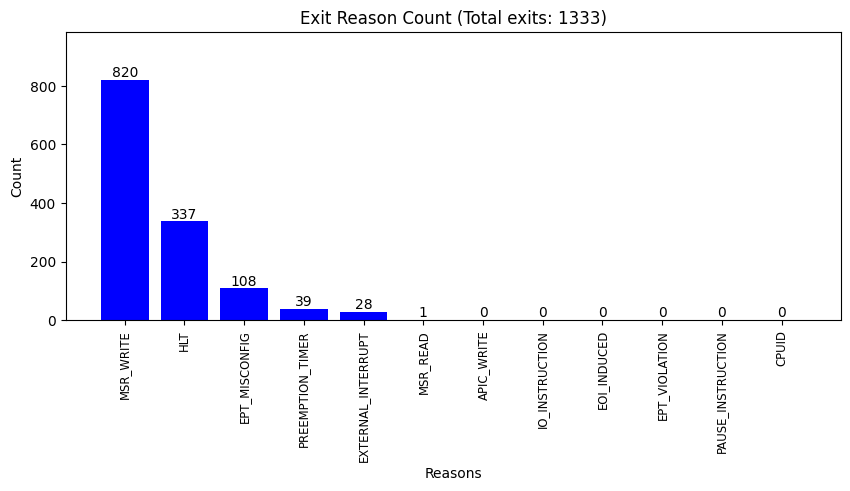
\includegraphics[width=1.0\columnwidth]{img/kvm_exit_vapic.png}
	\caption[kvm exits default]{kvm exits default}
	\label{fig:kvm_exit_vapic}
\end{figure}
\clearpage

\clearpage
\subsection{HLT}

\clearpage
\subsection{EPT\_MISCONFIG}

\clearpage
\subsection{PREEMPTION\_TIMER}

\clearpage
\subsection{EXTERNAL\_INTERRUPT}

\clearpage
\subsection{IO\_INSTRUCTION}

\clearpage
\subsection{EOI\_INDUCED}

\clearpage
\subsection{EPT\_VIOLATION}

\clearpage
\subsection{PAUSE\_INSTRUCTION}

\clearpage
\subsection{CPUID}

\clearpage
\subsection{MSR\_READ}

\clearpage

\chapter{Real-Time Performance Tuning}\label{cha:real-time_tuning}
\section{BIOS Configurations}
\section{Kernel Configurations} 
\section{Host OS Configurations}
\subsection{Tasks and Events}
\clearpage
\subsection{CPU governor}

Figure \ref{fig:power_saver_kvm_exit} shows ...

\begin{figure}[H]
	\centering
	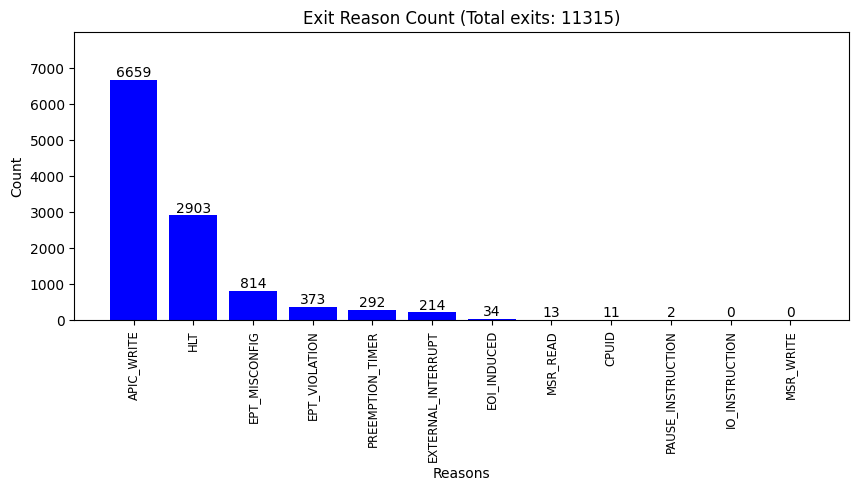
\includegraphics[width=1.0\columnwidth]{img/power_saver/kvm_exit_count.png}
	\caption[power\_saver kvm\_exit\_count]{power\_saver kvm\_exit\_count}
	\label{fig:power_saver_kvm_exit}
\end{figure}
\clearpage

Figure \ref{fig:power_saver_kvm_host} shows ...

\begin{figure}[H]
	\centering
	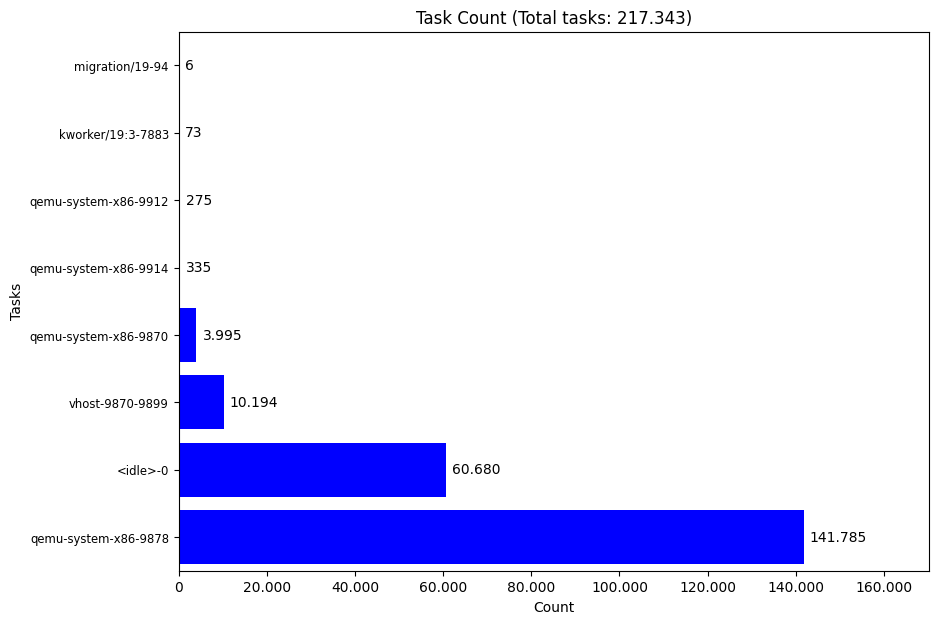
\includegraphics[width=1.0\columnwidth]{img/power_saver/results_host_report.png}
	\caption[power\_saver host report]{power\_saver host report}
	\label{fig:power_saver_kvm_host}
\end{figure}
\clearpage

Figure \ref{fig:power_saver_kvm_guest} shows ...

\begin{figure}[H]
	\centering
	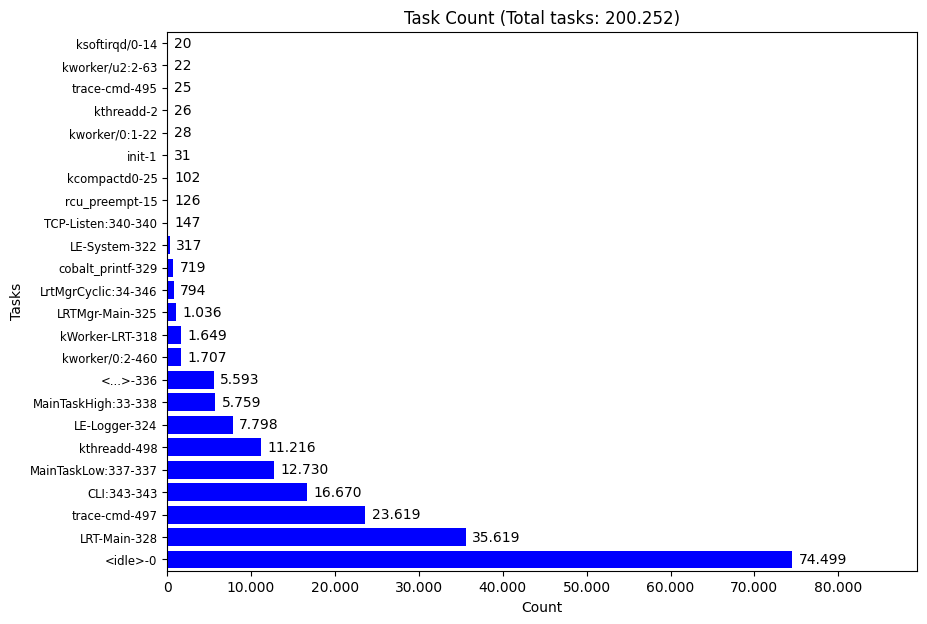
\includegraphics[width=1.0\columnwidth]{img/power_saver/results_guest_report.png}
	\caption[power\_saver guest report]{power\_saver guest report}
	\label{fig:power_saver_kvm_guest}
\end{figure}
\clearpage



Figure \ref{fig:balanced_kvm_exit} shows ...

\begin{figure}[H]
	\centering
	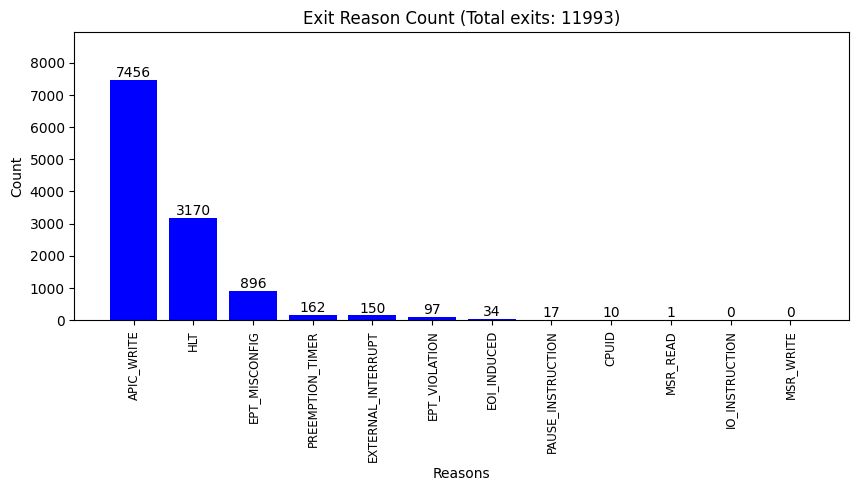
\includegraphics[width=1.0\columnwidth]{img/balanced/kvm_exit_count.png}
	\caption[balanced kvm\_exit\_count]{balanced kvm\_exit\_count}
	\label{fig:balanced_kvm_exit}
\end{figure}
\clearpage

Figure \ref{fig:balanced_kvm_host} shows ...

\begin{figure}[H]
	\centering
	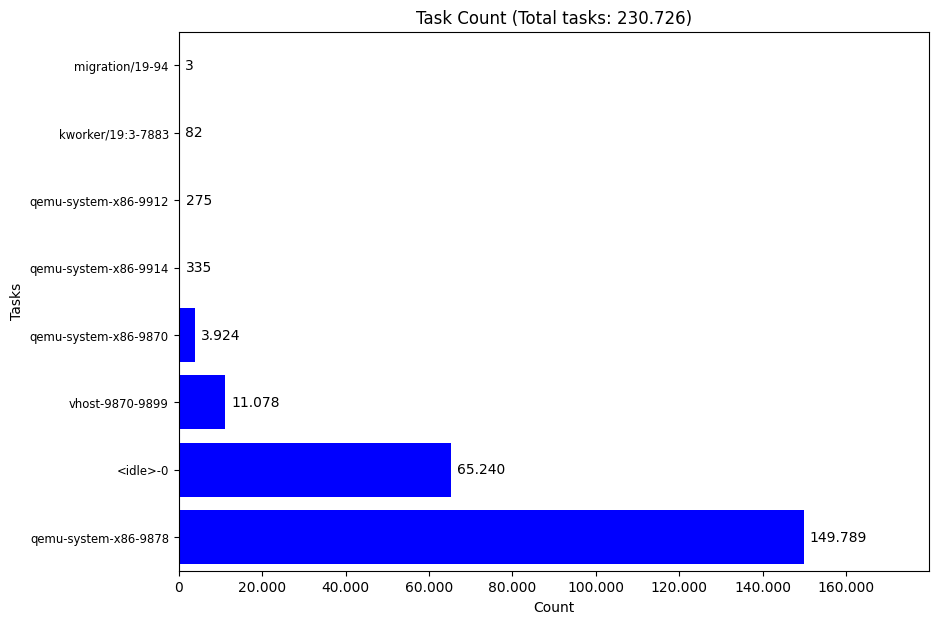
\includegraphics[width=1.0\columnwidth]{img/balanced/results_host_report.png}
	\caption[balanced host report]{balanced host report}
	\label{fig:balanced_kvm_host}
\end{figure}
\clearpage

Figure \ref{fig:balanced_kvm_guest} shows ...

\begin{figure}[H]
	\centering
	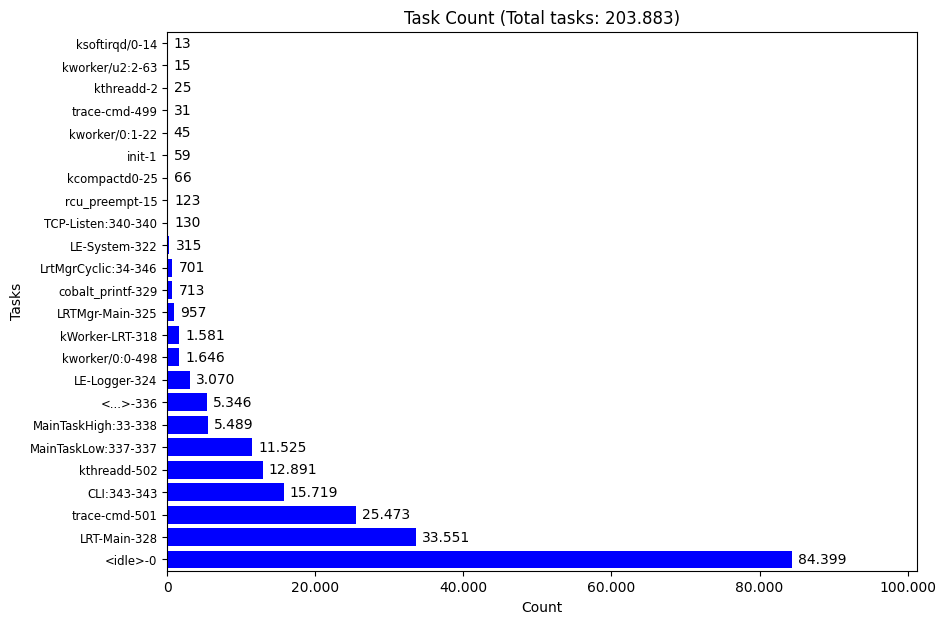
\includegraphics[width=1.0\columnwidth]{img/balanced/results_guest_report.png}
	\caption[balanced guest report]{balanced guest report}
	\label{fig:balanced_kvm_guest}
\end{figure}
\clearpage



Figure \ref{fig:performance_kvm_exit} shows ...

\begin{figure}[H]
	\centering
	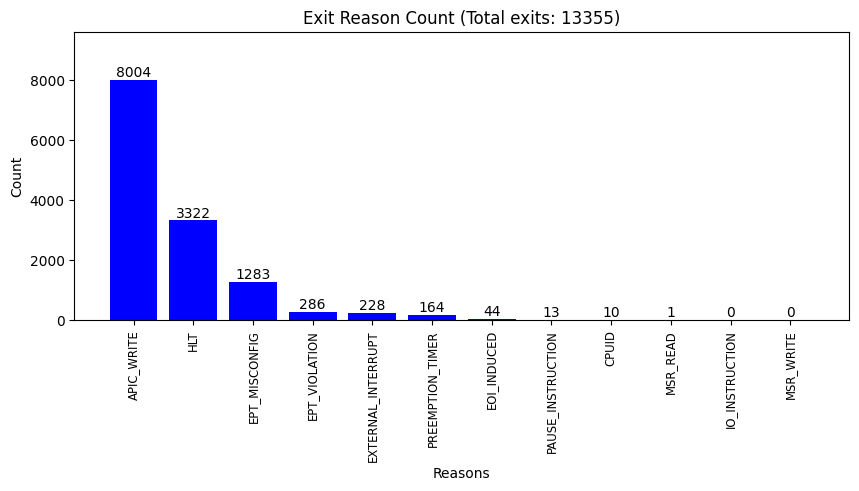
\includegraphics[width=1.0\columnwidth]{img/performance/kvm_exit_count.png}
	\caption[performance \_exit\_count]{performance \_exit\_count}
	\label{fig:performance_kvm_exit}
\end{figure}
\clearpage


Figure \ref{fig:performance_kvm_host} shows ...

\begin{figure}[H]
	\centering
	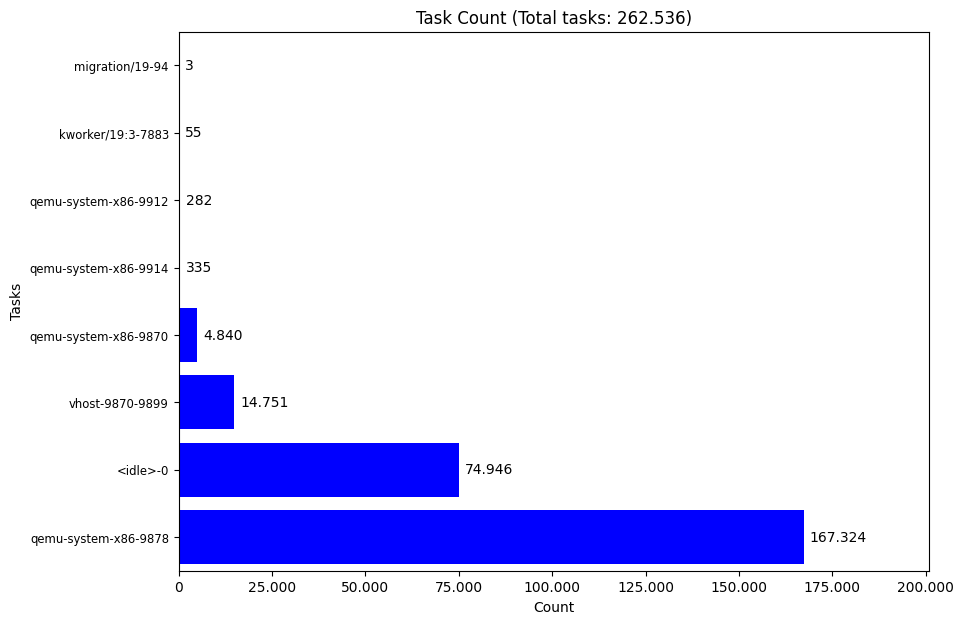
\includegraphics[width=1.0\columnwidth]{img/performance/results_host_report.png}
	\caption[performance host report]{performance host report}
	\label{fig:performance_kvm_host}
\end{figure}
\clearpage

Figure \ref{fig:performance_kvm_guest} shows ...

\begin{figure}[H]
	\centering
	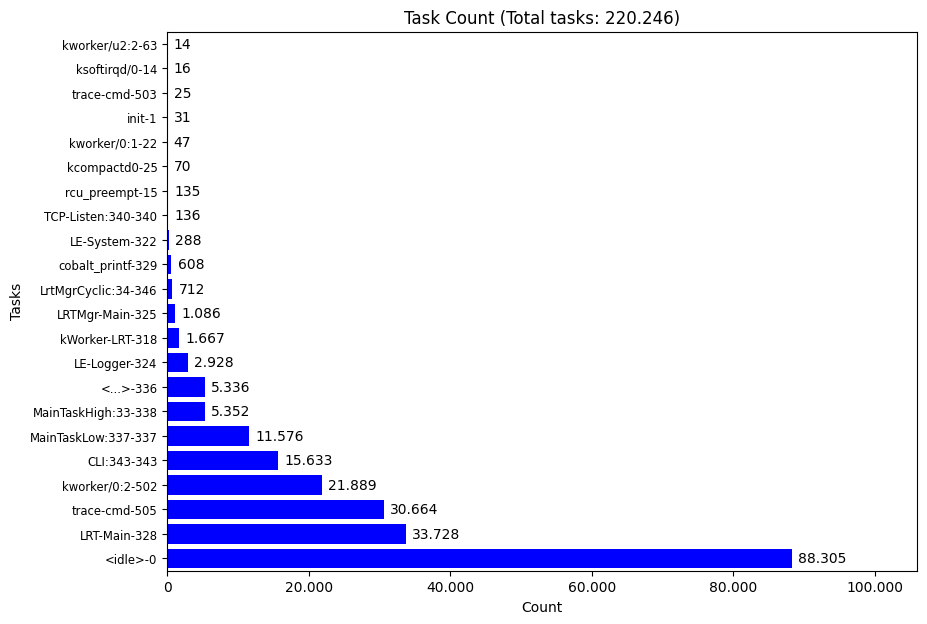
\includegraphics[width=1.0\columnwidth]{img/performance/results_guest_report.png}
	\caption[balanced guest report]{balanced guest report}
	\label{fig:performance_kvm_guest}
\end{figure}
\clearpage

\begin{comment}
\noindent Without CPU isolation, context switches take place at operating system level and not at hypervisor level. This explains why there are fewer \texttt{kvm\_exit} events. However, this will also, as previously shown, lead to higher latency, as context switches at operating system level generally take longer than a \texttt{kvm\_exit} and kvm\_entry.

\noindent When the CPU was dedicated to the QEMU process, on the other hand,there was a significant increase in \texttt{kvm\_exit} events. This is because every context switch takes place at hypervisor level. Nevertheless, lower latency was achieved thereby, as the qemu process is no longer influenced by the CPU scheduling of the operating system.
\end{comment}

\noindent In the process of analyzing the \texttt{kvm\_exit} events, several reasons for these exits were identified. The most frequent among these were the \texttt{APIC\_WRITE} and \texttt{HLT} events. The former is initiated when the guest writes to its Advanced Programmable Interrupt Controller (APIC), a component of the CPU that manages hardware interrupts. The latter occurs when the guest executes the HLT instruction, effectively halting the CPU until the next external interrupt is fired. Other significant but less frequent events included \texttt{EXTERNAL\_INTERRUPT} and \texttt{IO\_INSTRUCTION}. These events are indicative of the guest's interaction with hardware devices and its execution of I/O operations. Events such as \texttt{EPT\_MISCONFIG} and \texttt{PREEMPTION\_TIMER} were also noted. These could potentially signal issues with memory management and the host's scheduling of the guest. While events like \texttt{PAUSE\_INSTRUCTION}, \texttt{EPT\_VIOLATION}, \texttt{EOI\_INDUCED}, \texttt{MSR\_READ}, and \texttt{CPUID} were the least frequent, they still provide valuable insights into the guest's behavior and the host-guest interaction.

The gnuplot latency is visible in Figure \ref{fig:gnuplot_max_latency_hardware}
\begin{figure}[H]
	\centering
	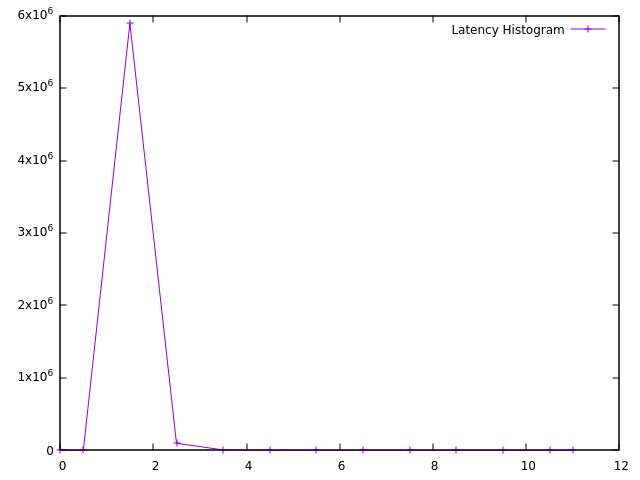
\includegraphics[width=0.8\columnwidth]{masterthesis-documentation/docs/sigmatek/xenomai/hardware/gnuplot_max_latency_hardware.png}
	\caption[gnuplot latency hardware]{gnuplot latency hardware}
	\label{fig:gnuplot_max_latency_hardware}
\end{figure}

Figure \ref{fig:gnuplot_max_latency_default}
\begin{figure}[H]
	\centering
	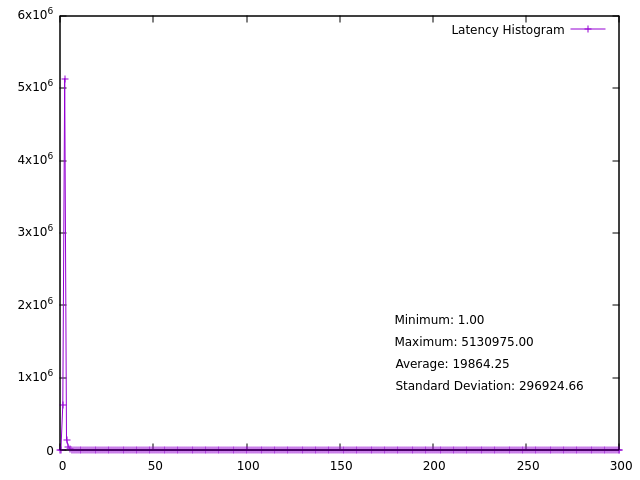
\includegraphics[width=0.8\columnwidth]{masterthesis-documentation/docs/sigmatek/xenomai/default/gnuplot_max_latency_default.png}
	\caption[gnuplot latency no taskset]{gnuplot latency no taskset}
	\label{fig:gnuplot_max_latency_default}
\end{figure}

Figure \ref{fig:gnuplot_max_latency_taskset}
\begin{figure}[H]
	\centering
	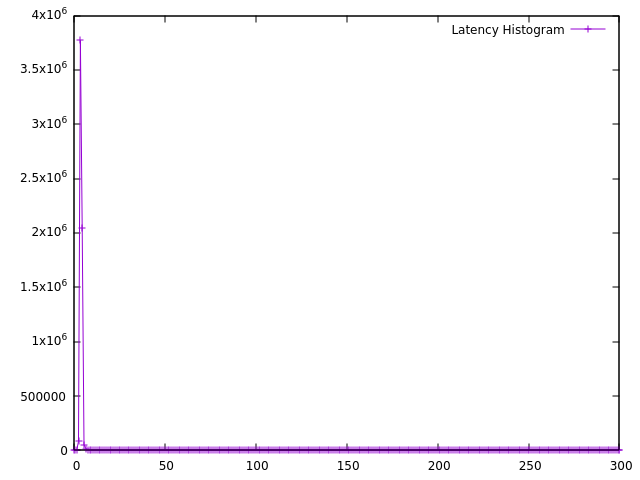
\includegraphics[width=0.8\columnwidth]{masterthesis-documentation/docs/sigmatek/xenomai/taskset/gnuplot_max_latency_taskset.png}
	\caption[gnuplot latency with taskset]{gnuplot latency with taskset}
	\label{fig:gnuplot_max_latency_taskset}
\end{figure}

Figure \ref{fig:gnuplot_max_latency_vapic}
\begin{figure}[H]
	\centering
	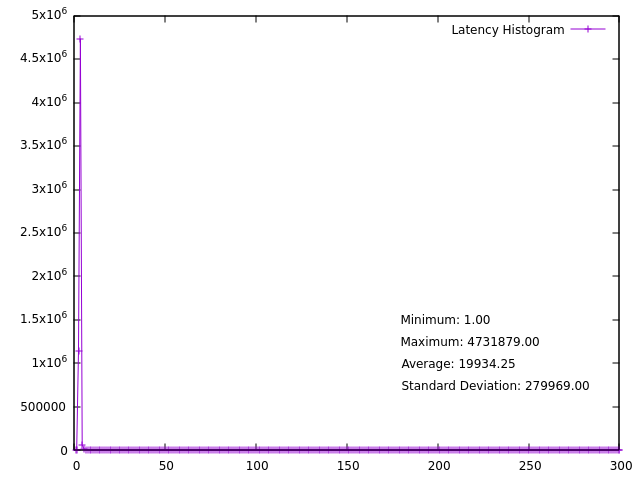
\includegraphics[width=0.8\columnwidth]{masterthesis-documentation/docs/sigmatek/xenomai/vapic/gnuplot_max_latency_vapic.png}
	\caption[gnuplot latency with taskset]{gnuplot latency with taskset}
	\label{fig:gnuplot_max_latency_vapic}
\end{figure}


\clearpage
\subsection{CPU isolation}
Isolating CPUs involves removing all user-space threads and unbound kernel threads since bound kernel threads are tied to specific CPUs and hence cannot be moved. Also, modifying the \texttt{proc/irq/IRQ\_NUMBER/smp\_affinity} property of each Interrupt IRQ\_NUMBER in the system is part of this process, as described later in section \ref{sec:irq_handling}. Output \ref{output:pse} shows the user and kernel tasks that run on CPU 19. After the isolation, user tasks other than the QEMU process have been removed from running on this CPU. Only few critical kernel threads that are tied to this CPU still take CPU time.

\vspace{1em}
\begin{minipage}{0.95\columnwidth}
	\begin{lstlisting}[name={User and Kernel Tasks},label={output:pse},escapeinside={(*@}{@*)}]
		sigma_ibo@sigma-ibo:~$ cat /sys/devices/system/cpu/isolated
		19
		sigma_ibo@sigma-ibo:~$ ps -e -o pid,psr,comm | awk '$2 == 19'
				92  19 cpuhp/19
				93  19 idle_inject/19
 	    		94  19 migration/19
 	    		95  19 ksoftirqd/19
 	    		97  19 kworker/19:0H-events_highpri
 	 		 1025  19 irq/205-iwlwifi:queue_7
 	 		17448  19 kworker/19:1H-kblockd
 	 		17499  19 kworker/19:2-events
 	 		18761  19 kworker/19:3-events
			21401  19 qemu-system-x86
\end{lstlisting}
\end{minipage}

\clearpage
\subsection{Interrupt Requests Handling}\label{sec:irq_handling}
Once the CPUs were isolated, Interrupt Requests Handling was the next step. Interrupt Requests are used to send a signal to the CPU, prompting it to 'interrupt' its current task and divert its attention to another task. This allows hardware devices to communicate with the CPU through frequent context switches, which can lead to performance degradation, especially in high-performance computing or real-time scenarios. To mitigate this, the IRQs needed to be removed from the isolated CPUs. This was done by manipulating a file in the proc filesystem, namely \texttt{/proc/irq/<IRQ>/smp\_affinity}. The value in the \texttt{smp\_affinity} file is a bitmask in hexadecimal format. Each bit in this mask corresponds to a CPU in the system. The least significant bit (LSB) on the right corresponds to the first CPU (CPU0), and the significance increases towards the left until CPU19. In a system with 20 CPUs, if every CPU was reserved for one IRQ, the value for \texttt{smp\_affinity} would be FFFFF. The script in code \ref{script:smp_affinity} was written to check and log the distribution of Interrupt Requests across each CPU in Salamander 4.

\vspace{1em}
\begin{minipage}{0.95\columnwidth}
	\begin{lstlisting}[name={Check distribution of Interrupt Requests across each CPU},label={script:smp_affinity}]
		#!/bin/bash
		# Check if a command-line argument is provided
		if [ -z "$1" ]; then
			echo "Please provide a CPU number as a command-line argument."
			exit 1
		fi
		# Get the CPU number from the command-line argument
		CPU=$1
		# Initialize an empty array to store the IRQ numbers
		IRQs=()
		for IRQ in /proc/irq/*; do
			if [ -f "$IRQ/smp_affinity" ]; then
				# Read the current smp_affinity
				AFFINITY=$(cat "$IRQ/smp_affinity")
				# Check if the bit for the current CPU is set
				if (( (0x$AFFINITY & (1 << CPU)) != 0 )); then
					# Add the IRQ number to the array
					IRQs+=("${IRQ#/proc/irq/}")
				fi
			fi
		done
		# Sort the array
		IFS=$'\n' sorted=($(sort -n <<<"${IRQs[*]}"))
		# Print the CPU number
		echo "CPU $CPU IRQ affinity:"
		# Print the sorted IRQ numbers on separate lines
		for irq in "${sorted[@]}"; do
			echo "$irq"
		done
		
\end{lstlisting}
\end{minipage}

Output \ref{output:irq_affinity} shows the output of the script above for CPU 19.

\vspace{1em}
\begin{minipage}{0.95\columnwidth}
\begin{lstlisting}[name={Output of smp_affinity for CPU 19},label={output:irq_affinity}, breaklines=true]
	sigma_ibo@sigma-ibo:~$ ./check_smp_affinity.sh 19
	CPU 19 IRQ affinity:
	0
	2
	3
	4
	5
	6
	7
	10
	11
	13
	15
	131
	172
	188
	189
	195
\end{lstlisting}
\end{minipage}


\noindent By changing the values of the \texttt{smp\_affinity} files of the respective IRQs, the assignment of IRQs was controlled so that they would not be handled by the isolated CPU. This reduced the interruptions caused by IRQs and the isolated CPUs were able to focus more on their assigned tasks.
\clearpage
\subsection{Real-time patch}
\clearpage
\section{QEMU-KVM Configurations}
\section{Guest OS Configurations}
\clearpage
\subsection{Tasks and Events}
\clearpage


\vspace{1em}
\begin{minipage}{\linewidth}
	\begin{lstlisting}[name={QEMU script for starting Salamander 4 virtualisation},label={script:qemu_configuration_optimizations}]
    #!/bin/sh

    if  [ ! -d drive-c/ ]; then
            echo "Filling drive-c/"
            mkdir drive-c/
            tar -C drive-c/ -xf stek-drive-c-image-sigmatek-core2.tar.gz
    fi
    
    exec  qemu-system-x86_64 -M pc,accel=kvm -kernel ./bzImage \
    -m 2048 -drive file=salamander-image-sigmatek-core2.ext4,format=raw,media=disk \
    -append "console=ttyS0 console=tty1 root=/dev/sda rw panic=1 sigmatek_lrt.QEMU=1 ip=dhcp rootfstype=ext4 schedstats=enable" \
    -net nic,model=e1000,netdev=e1000 -netdev bridge,id=e1000,br=nm-bridge \
    -fsdev local,security_model=none,id=fsdev0,path=drive-c -device virtio-9p-pci,id=fs0,fsdev=fsdev0,mount_tag=/mnt/drive-C \
    -device vhost-vsock-pci,guest-cid=3,id=vsock0 \
    -drive if=pflash,format=qcow2,file=ovmf.code.qcow2 \
    -no-reboot -nographic
\end{lstlisting}
\end{minipage}
\clearpage

Configurations for guest OS in the real-time VM .......................................................... 13


\chapter{Real-Time Robotic Application}\label{cha:real-time-testing}

\section{VARAN}
\clearpage
\section{Robotic Application}
\clearpage

\chapter{To Include}\label{cha:to_include}

The Figure \ref{fig:latency_comparison} below compares non-optimized guest latency with optimized guest latency and includes optimized bare-metal latency as a reference. The data shows that a 40\% reduction in QD1 latency is achievable through system tuning.

\begin{figure}[H]
	\centering
	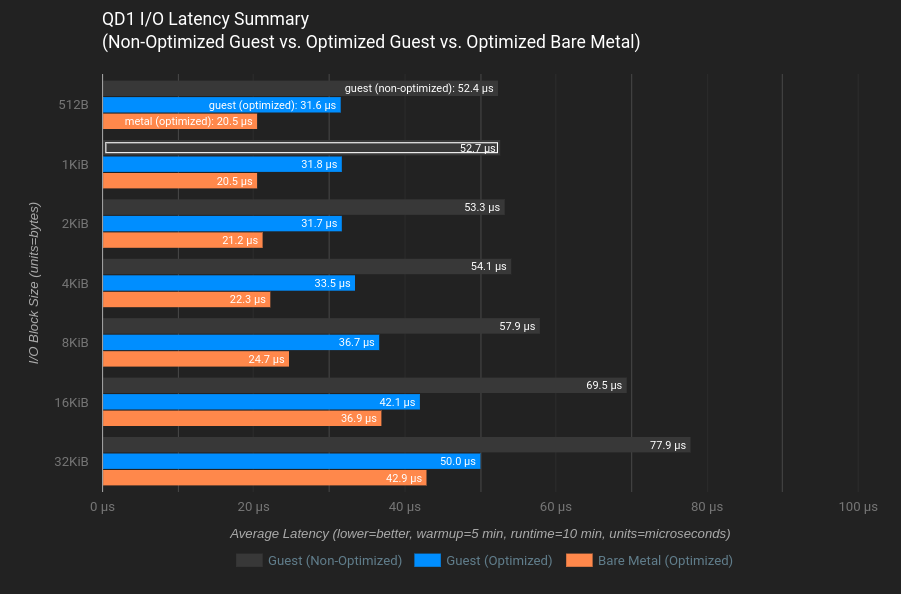
\includegraphics[width=1.0\columnwidth]{img/latency_comparison.png}
	\caption[latency comparison]{latency comparison}
	\label{fig:latency_comparison}
\end{figure}
\clearpage


\cite{pixelartSIGMATEKKompletteAutomatisierungssysteme}
\cite{Tracecmd}
\cite{KernelShark}
\cite{XenomaiXenomai}
\cite{WelcomeYoctoProject}
\cite{QEMU}
\cite{linPerformanceEvaluationXenomai}
\cite{abediRTNFPredictableLatency2019}
\cite{broskyShieldedProcessorsGuaranteeing2003}
\cite{casiniLatencyAnalysisVirtualization2021}
\cite{cinqueVirtualizingMixedCriticalitySystems2022}
\cite{garcia-vallsChallengesRealtimeVirtualization2014}
\cite{guStateoftheArtSurveyRealTime2012}
\cite{HardRealTime}
\cite{javierperezHowRealTime2022}
\cite{kirovaImpactModernVirtualization2019}
\cite{kiszkaLinuxRealTimeHypervisor}
\cite{lutsykPipelinedMulticoreMachine2020}
\cite{malallahComprehensiveStudyKernel2021}
\cite{masrurVMBasedRealTimeServices2010}
\cite{mckenneyRealTimeVs}
\cite{pielAsymmetricSchedulingLoad2006}
\cite{queirozTestingLimitsGeneralpurpose2023}
\cite{reghenzaniRealTimeLinuxKernel2020}
\cite{yoonRealTimePerformanceAnalysis}
\cite{adamPerformanceAssessmentLinux2021}
\clearpage

\chapter{Results}\label{cha:results}

\begin{comment}

VARAN-Bus PCV-521\newline
Windows\newline
Ubuntu\newline
WSL\newline\newline\newline



In Xenomai 3, you need:

The Linux kernel with the Dovetail interface, which allows the kernel to handle real-time tasks with low latency.
The Cobalt real-time core, which is responsible for scheduling and executing real-time tasks.
In Xenomai 4, you need:
The Linux kernel with the EVL interface, which, like Dovetail, enables the kernel to handle real-time tasks with low latency.
The libevl library, which provides a user interface to the EVL core, allowing applications to use the real-time capabilities provided by EVL.
So, while both versions require a Linux kernel with a real-time interface (Dovetail for Xenomai 3, EVL for Xenomai 4), Xenomai 3 uses a real-time core (Cobalt), while Xenomai 4 uses a library (libevl) to provide applications with access to its real-time capabilities.
\end{comment}
\clearpage

\chapter{Discussion}\label{cha:discussion}
\clearpage

\chapter{Summary and Outlook}\label{cha:summary_and_outlook}

%
% Hier beginnen die Verzeichnisse.
%
\clearpage
\printbibliography
\clearpage

% Das Abbildungsverzeichnis
\listoffigures
\clearpage

% Das Tabellenverzeichnis
\listoftables
\clearpage

% Das Quellcodeverzeichnis
\listofcode
\clearpage

\phantomsection
\addcontentsline{toc}{chapter}{\listacroname}

\chapter*{\listacroname}
\begin{acronym}[XXXXX]
	\acro{CPU}[CPU]{Central Processing Unit}
	\acro{QEMU}[QEMU]{Quick Emulator}
	\acro{IRQ}[IRQ]{Interrupt Request}
\end{acronym}

%
% Hier beginnt der Anhang.
%
\clearpage
\appendix

\chapter{Anhang A}
\clearpage

\chapter{Anhang B}

\end{document}